\documentclass {leaflet}


\renewcommand*\foldmarkrule{.3mm}
\renewcommand*\foldmarklength{5mm}

\usepackage[T1]{fontenc}
\usepackage{textcomp}
\usepackage{mathptmx}
\usepackage[scaled=0.9]{helvet}
\makeatletter
\def\ptmTeX{T\kern-.1667em\lower.5ex\hbox{E}\kern-.075emX\@}
\DeclareRobustCommand{\ptmLaTeX}{L\kern-.3em
        {\setbox0\hbox{T}%
         %\vb@xt@ % :-)
         \vbox to\ht0{\hbox{%
                            \csname S@\f@size\endcsname
                            \fontsize\sf@size\z@
                            \math@fontsfalse\selectfont
                            A}%
                      \vss}%
        }%
        \kern-.12em
        \ptmTeX}
\makeatother
\let\TeX=\ptmTeX
\let\LaTeX=\ptmLaTeX
\usepackage{shortvrb}
\MakeShortVerb{\|}
\usepackage{url}
\usepackage{graphicx}
\usepackage[dvipsnames,usenames]{color}
\definecolor{LIGHTGRAY}{gray}{.9}

%%%%\renewcommand{\descfont}{\normalfont}
\newcommand\Lpack[1]{\textsf{#1}}
\newcommand\Lclass[1]{\textsf{#1}}
\newcommand\Lopt[1]{\texttt{#1}}
\newcommand\Lprog[1]{\textit{#1}}

\newcommand*\defaultmarker{\textsuperscript\textasteriskcentered}

\title{Workshop on Innovations in University Mathematics Teaching\\
7th to 8th July 2014}
\author{}
\date{}

\CutLine*{1}% Dotted line without scissors
\CutLine*{3}% Dotted line without scissors
\CutLine*{4}% Dotted line without scissors
\CutLine*{6}%  Dotted line with scissors

\AddToBackground{1}{%  Background of a small page
  \put(0,0){\textcolor{LIGHTGRAY}{\rule{\paperwidth}{\paperheight}}}}
\AddToBackground{3}{%  Background of a small page
  \put(0,0){\textcolor{LIGHTGRAY}{\rule{\paperwidth}{\paperheight}}}}
\AddToBackground{5}{%  Background of a small page
  \put(0,0){\textcolor{LIGHTGRAY}{\rule{\paperwidth}{\paperheight}}}}

\begin{document}

\maketitle
\thispagestyle{empty}

\begin{center}
{\Large Cardiff University}\\
\vspace{1cm}
Flipped Classroom \textbf{and} Inquiry Based Learning\\
\vspace{1cm}
{\Large\url{mathsevents.cf.ac.uk/mathedworkshop}}\\
\vspace{3cm}

\includegraphics[width=.4\textwidth]{./Images/universitylogo.eps}
\hspace{.1\textwidth}

\includegraphics[width=.4\textwidth]{./Images/wimcslogo.jpg}
\end{center}

\newpage
\section{Description}
\vspace{1cm}

This 2-day workshop will introduce delegates to innovative approaches to
teaching mathematics in university settings. In particular there will
be masterclasses on two methods: inquiry based learning and flipped
classrooms, combined with plenty of opportunities for delegates to
experience these methods in practice and reflect on ways in which they
might be embedded within their own teaching. We are delighted to have
expert speakers from the UK and US share with us how they are using such
methods within their own teaching.\\

\vspace{1cm}

\textbf{Inquiry based learning} focuses attention on the student's role in making sense of mathematical ideas for himself or herself, and communicating those ideas clearly to peers. Students are given tasks requiring them to solve problems, conjecture, experiment, explore, create, and communicate... all those wonderful skills and habits of mind that Mathematicians engage in regularly. Rather than showing facts or a clear, smooth path to a solution, the instructor guides and mentors students via well-crafted problems through an adventure in mathematical discovery.\\

\vspace{1cm}
\textbf{A flipped classroom} is a model in which students gain first-exposure learning prior to class and focus on the processing part of learning (synthesizing, analyzing, problem-solving, etc.) in class. It aims to modify the locus of content delivery so as to ensure that contact time is student centered. This methodology often makes use of modern technological tools but does not require them.

\newpage
\section{Schedule}
\subsection{7th of July}
\vspace{1cm}

\textbf{Session 1}\\

10.20 - 10.30 : \textit{Welcome and introduction} (Paul Harper)\\
10.30 - 11.30 : \textit{Flipping the University Mathematics Classroom: A Gateway to Lifelong Learning} (Robert Talbert)\\
11.30 - 12.00: \textit{Using a Flipped Classroom in a Large Programming Course for Mathematicians} (Vince Knight)\\
12.00 - 12.30 : \textit{TBC} (Toby Bailey)\\

\textbf{Lunch} (12.30 - 13.15)\\

\textbf{Session 2}\\

13.15 - 13.45 : \textit{TBC} (Chris Sangwen)\\
13.45 - 14.15 : \textit{TBC} (Steve Rutherford)\\
14.15 - 14.45 : \textit{Panel discussion on flipped classrooms}\\

\textbf{Session 3}\\

15.00 - 16.30 : \textit{Inquiry-Based Education in Mathematics: Models, Methods, and Effectiveness for Higher Education (Part 1)} (Theron Hitchman \& Dana Ernst)\\

\textbf{Workshop dinner} (from 19.00)

\newpage
\section{Schedule}
\subsection{8th of July}
\vspace{1cm}

\textbf{Session 4}

09.30 - 13.00 : \textit{Inquiry-Based Education in Mathematics: Models, Methods, and Effectiveness for Higher Education (Part 2)} (Theron Hitchman \& Dana Ernst)\\

\textbf{Lunch} (13.00 - 13.45)\\

13.45 - 15.15: \textit{Teaching Cafe: encouraging delegates to discuss how some of the methodologies presented could be used in their own classes.}\\

15.15 : \textit{Closing remarks}

\newpage
\section{Location}
\vspace{1cm}

The workshop will take place in the School of Mathematics, Cardiff University, CF24 4AG.\\

\vspace{1cm}

\begin{center}
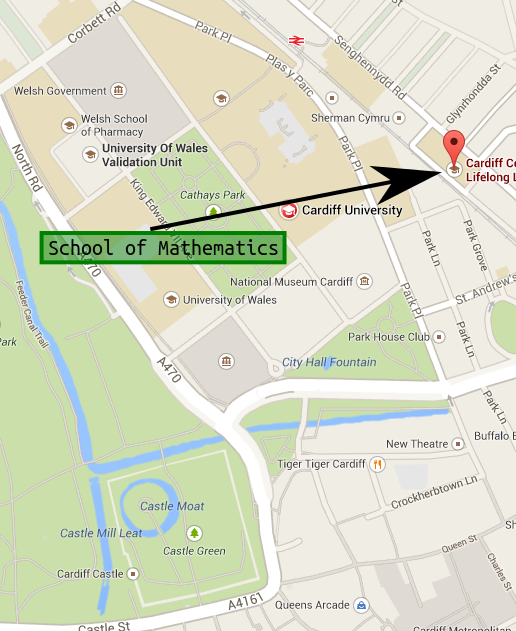
\includegraphics[width=.95\textwidth]{./Images/map.png}
\end{center}

\vspace{1cm}

There are many different accommodation options for a range of budgets within walking distance of the University. For more information please see the Visit Cardiff website:
\begin{center}
\url{www.visitcardiff.com}
\end{center}

\newpage
\section{Registration and Contacts}
\subsection{Registration fee}

The registration fee is just \pounds90 (we have tried to keep costs to a minimum and please note all fees will be used to cover the cost of the workshop). \\

This fee covers attendance for both days, \textbf{lunches and refreshments on both days, and dinner on the Monday evening}.\\


\subsection{Deadline}
Deadline for booking is \textbf{Friday 20th June}.\\

To book your place please see the booking page at:
\begin{center}
\url{mathsevents.cf.ac.uk/mathedworkshop}.
\end{center}

\subsection{Contacts}
For further information please don't hesitate to get in touch with the organisers:

\begin{center}
Paul Harper: \url{harper@cf.ac.uk}\\
Vince Knight: \url{knightva@cf.ac.uk}\\
Rob Wilson: \url{wilsonrh@cf.ac.uk}
\end{center}


\loggingall
\end{document}
\endinput
%%
%% End of file `leaflet-manual.tex'.
